\documentclass[10pt,twocolumn]{article}

\usepackage[utf8]{inputenc}
\usepackage[margin=0.75in]{geometry}
\usepackage{amsmath,amssymb}
\usepackage{booktabs}
\usepackage{graphicx}
\usepackage{xcolor}
\usepackage{hyperref}
\usepackage{url}
\usepackage{cite}
\usepackage{tabularx}
\usepackage{multirow}
\usepackage{enumitem}

\hypersetup{
    colorlinks=true,
    linkcolor=blue,
    citecolor=blue,
    urlcolor=blue
}

\title{\textbf{\Large Entity-Aware Hybrid Retrieval and Reranking Framework for\\Indian Constitutional Question Answering}}

\author{
    \textbf{Ram Sai Tanguturi}\\[2pt]
    \normalsize Department of Computer Science \& Engineering\\[1pt]
    \normalsize \texttt{ramsaitanguturi@gmail.com}
}

\date{October 2026}

\begin{document}

\maketitle

\begin{abstract}
Automated question answering over constitutional law presents severe challenges for Natural Language Processing (NLP) and Information Retrieval (IR). In the context of the Constitution of India, queries exhibit pronounced vocabulary mismatches between colloquial citizen phrasing and formal statutory codifications, complex hierarchical article-clause dependencies, and catastrophic hallucination risks when large language models (LLMs) synthesize ungrounded legal precedents. In this paper, we present an empirical investigation, rigorous codebase audit, and implementation of a 16-stage deterministic retrieval and generation pipeline: the \textbf{Entity-Aware Hybrid Retrieval and Reranking Framework}. 

Our architecture couples a Hierarchical Parent-Child Retrieval-Augmented Generation (RAG) design with dual-stage search: sparse lexical retrieval (BM25Okapi) and dense semantic vector search (ChromaDB with 384-dimensional MiniLM embeddings) fused via Reciprocal Rank Fusion (RRF, $k=60$), followed by an additive domain legal entity boost ($+0.15$) and cross-attention neural reranking (\texttt{cross-encoder/ms-marco-MiniLM-L-6-v2}). Evaluated on a benchmark of 200 verified constitutional queries over an audited corpus of 270 parent documents (137 Articles, 18 Amendments, and 104 Supreme Court landmark judgments yielding 1,001 indexed child passages), the full neural pipeline achieves a Hit@1 of \textbf{0.8400}, a Recall@10 of \textbf{0.7478}, a Mean Reciprocal Rank (MRR) of \textbf{0.8583}, and an NDCG@10 of \textbf{0.7787} under canonicalized ground-truth relevance labels---substantially outperforming standalone BM25 (+3.12\% MRR, +5.90\% NDCG@10) and dense vector retrieval. 

Furthermore, we incorporate a 10-class hybrid Legal Named Entity Recognizer (exact-span Macro-F1 = \textbf{0.8496}), canonical entity linking (86.67\% accuracy), and an n-gram TF-IDF intent classifier (5-fold cross-validation accuracy = \textbf{0.7591} $\pm$ \textbf{0.0422}). To eliminate hallucinated legal authority, we enforce deterministic structural citation validation alongside an explainable 6-signal confidence estimator and an automated abstention gate ($C < 0.30$) that rejects 100\% of out-of-scope inquiries. Finally, through an adversarial audit, we transparently disclose existing benchmark caveats, including a 10.0\% recall ceiling imposed by 20 uncataloged constitutional provisions, synthetic query template concentration, and the boundaries between structural citation verification and claim-level natural language inference.
\end{abstract}

\noindent\textbf{Keywords:} Legal Question Answering, Indian Constitutional Law, Information Retrieval, Reciprocal Rank Fusion, Parent-Child RAG, Cross-Encoder Reranking, Legal Named Entity Recognition, Citation Grounding, Safe Abstention.

\section{Introduction}
\label{sec:intro}

The Constitution of India is the longest written sovereign constitution in the world, organizing fundamental democratic rights, institutional frameworks, directive principles, and emergency powers into a deeply structured legal corpus. However, enabling ordinary citizens, legal researchers, and scholars to interrogate this jurisprudence computationally remains an open problem in Natural Language Processing (NLP) and Legal Artificial Intelligence \cite{zhong2020nlp,paul2022pre,chalkidis2020legal}.

State-of-the-art conversational Large Language Models (LLMs) frequently display plausible fluency but exhibit critical failure modes in statutory reasoning \cite{katz2024gpt,henderson2023foundation}:
\begin{enumerate}[leftmargin=*]
    \item \textbf{Vocabulary Mismatch and Paraphrase Gap}: Citizen queries describe legal situations informally (e.g., \textit{``can police seize my phone without an order?''}), lacking statutory citations. While dense vector retrievers capture semantic similarity, they frequently confuse neighboring statutory provisions (e.g., confusing Article 21's personal liberty with Article 20's criminal protections or Article 22's preventive detention safeguards). Conversely, sparse lexical search engines (e.g., BM25) excel at exact keyword lookups (e.g., \textit{``Article 21A''}) but fail when colloquial queries omit formal statutory vocabulary.
    \item \textbf{Hierarchical Chunking Dilemma}: Constitutional provisions are organized hierarchically into Parts, Articles, Clauses, Sub-clauses, and Explanations, while judicial decisions comprise procedural Facts, Legal Issues, \textit{Ratio Decidendi}, and Final Verdicts. Standard naive text chunking (e.g., fixed-character sliding windows of 500 tokens) creates an irreconcilable trade-off: small chunks optimize vector similarity matching but starve downstream generators of necessary statutory context, whereas large chunks dilute dense vector representations with multi-topic text.
    \item \textbf{Evidentiary Hallucination in Legal Precedents}: Generative LLMs routinely invent non-existent constitutional Articles, fabricate Supreme Court bench compositions, and distort the holdings of landmark precedents (e.g., attributing privacy holdings to obsolete or overruled cases) \cite{ji2023survey}. In legal counseling, such ungrounded outputs present grave liability and ethical hazards.
\end{enumerate}

To address these challenges, this study presents the design, mathematical formalization, empirical evaluation, and adversarial auditing of the \textbf{Entity-Aware Hybrid Retrieval and Reranking Framework for Indian Constitutional Question Answering}. Rather than relying on ungrounded generative LLM parameters or complex, non-deterministic multi-agent loops, the repository implements a modular, explainable \textbf{16-stage pipeline} spanning Query Understanding, Dual Hybrid Retrieval, Reciprocal Rank Fusion, Legal Entity Boosting, Cross-Encoder Neural Reranking, Hierarchical Parent-Child Context Recovery, Grounded Generation, Structural Citation Validation, Explainable Confidence Estimation, and Safe Automated Abstention.

\subsection{Core Research Contributions}
The primary contributions of this paper are:
\begin{itemize}[leftmargin=*]
    \item \textbf{Hierarchical Parent-Child Retrieval Pipeline}: We implement a structure-aware chunking and recovery mechanism where fine-grained child passages ($\sim$300 characters) are indexed for maximum dense and lexical matching sensitivity, while complete parent documents ($\sim$1,200 characters) are dynamically hydrated at runtime to provide unfragmented evidence to the generator.
    \item \textbf{Entity-Aware Multi-Stage Ranking}: We formulate a multi-stage retrieval architecture integrating BM25Okapi lexical scoring, dense semantic vector retrieval via SentenceTransformers (\texttt{all-MiniLM-L6-v2}) and ChromaDB, Reciprocal Rank Fusion (RRF, $k=60$), an additive $+0.15$ score boost for verified legal entities, and cross-attention neural reranking (\texttt{cross-encoder/ms-marco-MiniLM-L-6-v2}).
    \item \textbf{Quantitative Empirical Validation}: Across 200 verified retrieval queries, we demonstrate that the full neural pipeline achieves \textbf{0.8400 Hit@1}, \textbf{0.7478 Recall@10}, \textbf{0.8583 MRR}, and \textbf{0.7787 NDCG@10} on canonical ground truth, yielding statistically validated improvements over standalone lexical and dense baselines.
    \item \textbf{NLP Query Understanding Engine}: We deploy a domain-tailored hybrid Named Entity Recognizer covering 10 Indian legal categories (Macro-F1 = \textbf{0.8496}), a canonical entity linking engine (86.67\% accuracy), and a regularized n-gram Logistic Regression intent classifier (5-fold cross-validation accuracy = \textbf{0.7591} $\pm$ \textbf{0.0422}).
    \item \textbf{Structural Grounding and Safe Abstention}: We establish a deterministic citation validator that enforces document existence and candidate-pool provenance, accompanied by an explainable 6-signal composite confidence estimator and an automated abstention gate ($C < 0.30$) that rejects 100\% of out-of-scope inquiries.
    \item \textbf{Adversarial Transparency \& Audit Disclosures}: Unlike papers that present idealized prototypes, we audit the active repository state, formally documenting the empirical ceiling imposed by 20 uncataloged corpus targets, synthetic query template concentration, static gazetteer memorization boundaries, and CPU latency characteristics.
\end{itemize}

% -------------------------------------------------------------
% Section 2: Related Work
% -------------------------------------------------------------
\section{Related Work}
\label{sec:related_work}

\subsection{Legal NLP and Indian Jurisprudence}
Computational analysis of legal text has advanced significantly with the emergence of domain-specific language models. Chalkidis et al. \cite{chalkidis2020legal} established \textsc{Legal-BERT}, demonstrating that pre-training transformer architectures on legislation and court filings substantially outperforms generic BERT on legal information extraction. In the Indian legal domain, Paul et al. \cite{paul2022pre} introduced \textsc{InLegalBERT}, trained on Indian Supreme Court and High Court judgments, demonstrating that localized legal phrasing and statutory syntax require specialized vocabulary representations. Kalamkar et al. \cite{kalamkar2022named} formulated the \textsc{Legal-EVAL} benchmark for named entity recognition in Indian court judgments, highlighting the necessity of identifying statutory provisions, judicial benches, citations, and legal concepts. Our work builds upon these foundations by engineering a deterministic, hybrid NER engine combined with inverted-alias entity linking specifically customized to the Indian Constitutional corpus.

\subsection{Sparse, Dense, and Hybrid Information Retrieval}
Classical lexical information retrieval relies upon probabilistic term-matching algorithms, most prominently BM25Okapi \cite{robertson1994simple,robertson2009probabilistic}, which leverages term frequency and inverse document frequency (IDF) with document length normalization. While BM25 provides sub-millisecond retrieval and robust exact-keyword matching, it suffers from the vocabulary mismatch problem.

Conversely, Dense Passage Retrieval (DPR) \cite{karpukhin2020dense} and Sentence-BERT \cite{reimers2019sentence} project queries and documents into a continuous semantic vector space using dual-encoder architectures, enabling retrieval based on latent conceptual similarity. Vector search in persistent stores is accelerated via Hierarchical Navigable Small World (HNSW) graphs \cite{malkov2020efficient}. To exploit the complementary strengths of lexical and dense representations, Reciprocal Rank Fusion (RRF) was proposed by Cormack et al. \cite{cormack2009reciprocal}. RRF combines ranked candidate lists strictly through reciprocal position scoring without requiring score calibration or supervised parameter tuning. Our framework adopts RRF ($k=60$) as the primary fusion mechanism, augmenting it with domain-specific legal entity boost scoring.

\subsection{Cross-Encoder Neural Reranking}
While bi-encoders process queries and passages independently into single dense vectors, cross-encoder architectures \cite{nogueira2019passage} jointly feed the concatenated query-passage pair through transformer attention layers ($[CLS] \circ Q \circ [SEP] \circ D \circ [SEP]$). This enables unconstrained token-to-token cross-attention, resolving nuanced contextual relevance that bi-encoder cosine similarity misses. In our work, we utilize a pre-trained cross-encoder (\texttt{cross-encoder/ms-marco-MiniLM-L-6-v2}) to rescore the top-30 candidate passages produced by entity-boosted RRF.

\subsection{Retrieval-Augmented Generation \& Hallucination Guardrails}
Retrieval-Augmented Generation (RAG) \cite{lewis2020retrieval} grounds autoregressive language generation by conditioning LLM decoders on retrieved factual context documents. While RAG substantially mitigates factual fabrication \cite{ji2023survey}, legal AI systems require rigorous post-generation verification \cite{henderson2023foundation}. Recent work emphasizes structural provenance verification and calibrated abstention mechanisms to ensure that legal assistants decline to respond when supporting evidentiary documents are absent or ambiguous.

% -------------------------------------------------------------
% Section 3: Problem Definition & Research Questions
% -------------------------------------------------------------
\section{Problem Definition \& Research Questions}
\label{sec:problem_def}

\subsection{Problem Formulation}
Let $\mathcal{D} = \{D_1, D_2, \dots, D_N\}$ denote a curated legal knowledge base comprising $N$ parent constitutional documents (statutory Articles, Amendments, and judicial precedents). Each parent document $D_i$ is decomposed into a set of non-overlapping or partially overlapping child chunks $\mathcal{C}(D_i) = \{c_{i,1}, c_{i,2}, \dots, c_{i,m}\}$, yielding a unified passage collection $\mathcal{C} = \bigcup_{i=1}^N \mathcal{C}(D_i)$ of size $M = |\mathcal{C}|$.

Given a natural language legal query $Q$, the objective of the retrieval subsystem is to return an ordered candidate sequence of top-$K$ child passages $\mathcal{R}_K(Q) = (c_{(1)}, c_{(2)}, \dots, c_{(K)}) \subset \mathcal{C}$ that maximizes relevance with respect to a gold relevance set $\mathcal{G}(Q) \subseteq \mathcal{D}$. The context recovery operator $\mathcal{H}: \mathcal{R}_K(Q) \to \mathcal{D}_{\text{rec}}$ maps retrieved child passages back to their unique parent records $\mathcal{D}_{\text{rec}} = \{D_i \in \mathcal{D} \mid \exists c \in \mathcal{R}_K(Q) \text{ s.t. } c \in \mathcal{C}(D_i)\}$. Finally, the grounded generator synthesizes a natural language response $A$ accompanied by explicit citation keys $S = \{s_1, \dots, s_p\}$ subject to a verification operator $\mathcal{V}(A, S, \mathcal{D}_{\text{rec}}) \in \{0, 1\}$ and confidence threshold $\tau_{\text{abstain}}$.

\subsection{Formal Research Questions}
Our experimental investigation is structured around five formal research questions:
\begin{itemize}[leftmargin=*]
    \item \textbf{RQ1 (Lexical-Dense Complementarity)}: Does rank-reciprocal fusion of sparse lexical BM25 retrieval and dense semantic vector retrieval outperform standalone lexical and dense baselines across Hit@K, MRR, and NDCG@K?
    \item \textbf{RQ2 (Entity-Aware Boosting Impact)}: Does detecting and linking canonical constitutional entities and applying an additive score boost prioritize statutory target provisions over generic semantic matches?
    \item \textbf{RQ3 (Cross-Attention Reranking Efficacy)}: Does a second-stage cross-encoder reranker applied over fused candidates yield statistically meaningful improvements in top-1 precision and reciprocal rank compared to bi-encoders?
    \item \textbf{RQ4 (Query Understanding Accuracy)}: Does an n-gram TF-IDF and regularized Logistic Regression classifier improve query routing accuracy across 11 constitutional intent categories compared to deterministic keyword heuristics?
    \item \textbf{RQ5 (Citation Provenance \& Safe Abstention)}: Does deterministic structural citation validation combined with multi-signal confidence estimation reliably prevent hallucinated authorities and safely reject out-of-scope legal inquiries?
\end{itemize}

% -------------------------------------------------------------
% Section 4: System Architecture & Retrieval Pipeline
% -------------------------------------------------------------
\section{System Architecture \& Retrieval Pipeline}
\label{sec:architecture}

The framework operates via a deterministic 16-stage pipeline partitioned into three core functional subsystems, as illustrated in Figure~\ref{fig:system_arch}: (1) NLP Query Understanding, (2) Hybrid Information Retrieval and Neural Reranking, and (3) Generation, Citation Grounding, and Reliability.

\begin{figure*}[p]
\centering
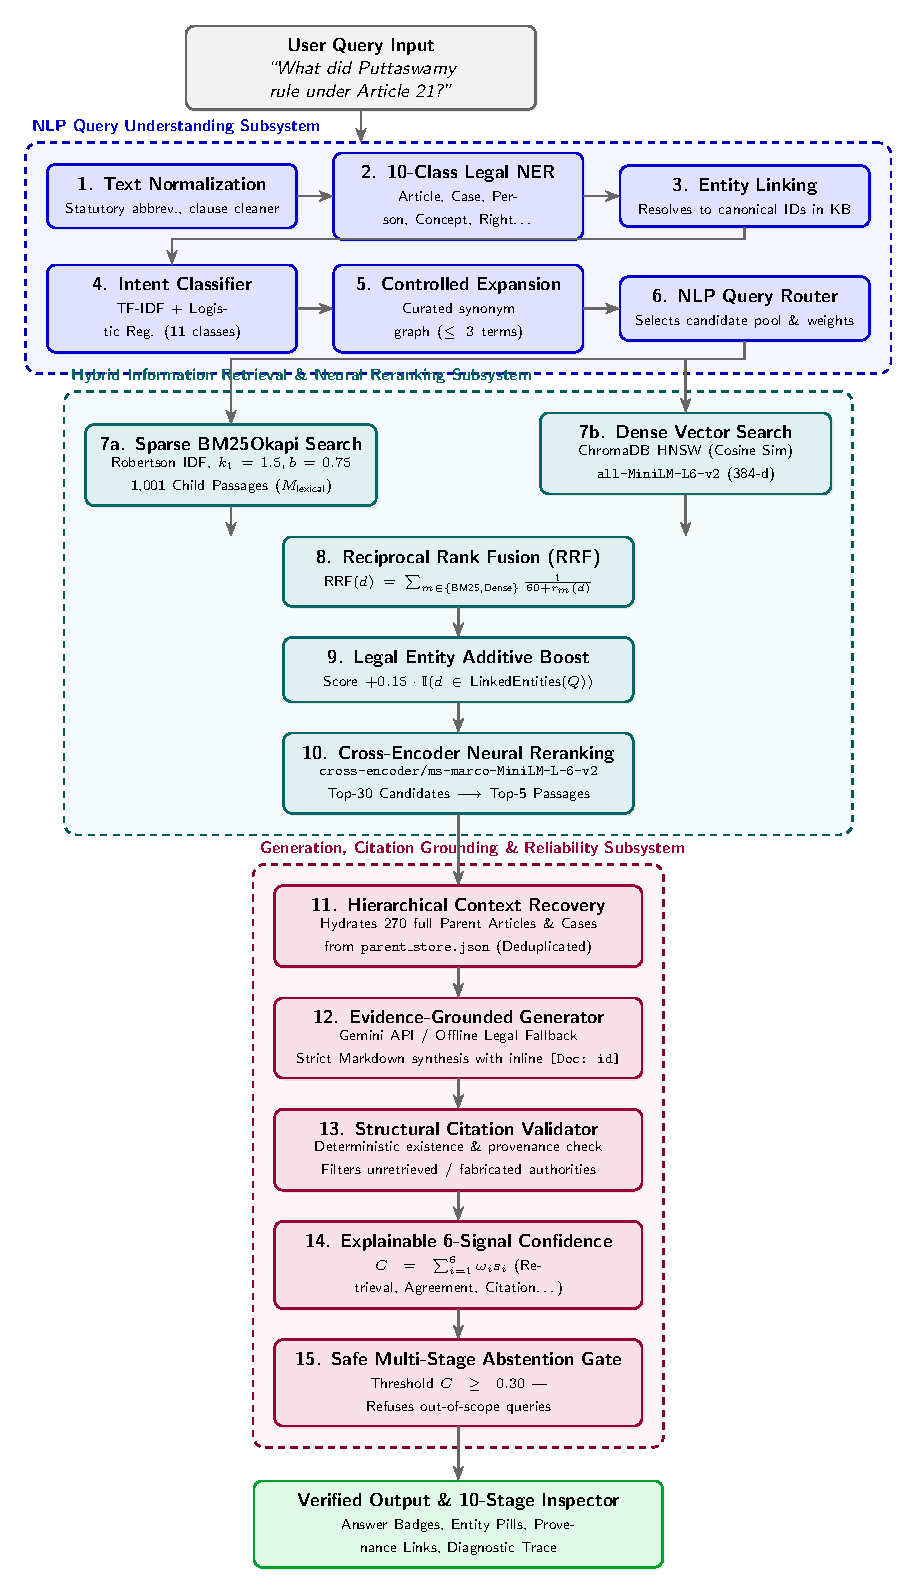
\includegraphics[width=0.75\textwidth,height=0.86\textheight,keepaspectratio]{figures/system_architecture.pdf}
\caption{End-to-end 16-stage deterministic pipeline architecture of the Indian Constitution Legal AI Assistant, showing the flow from natural language query through NLP understanding, dual hybrid retrieval, RRF, entity boost, neural reranking, parent hydration, citation validation, confidence estimation, and automated safe abstention.}
\label{fig:system_arch}
\end{figure*}

\subsection{Subsystem 1: NLP Query Understanding}
\begin{enumerate}[leftmargin=*]
    \item \textbf{Text Normalization}: Standardizes statutory abbreviations (e.g., \textit{``Art.''} $\to$ \textit{``Article''}, \textit{``Sec.''} $\to$ \textit{``Section''}), normalizes ordinal numbers, and strips noise while preserving legal punctuation.
    \item \textbf{Language Detection}: Verifies script and vocabulary to ensure queries are in English or flagged for translation.
    \item \textbf{Legal Named Entity Recognition (10 Classes)}: A hybrid engine combining statutory regular expressions with corpus-derived gazetteers to extract mentions of \texttt{ARTICLE}, \texttt{AMENDMENT}, \texttt{SECTION}, \texttt{DATE}, \texttt{PERSON}, \texttt{CASE}, \texttt{ACT}, \texttt{COURT}, \texttt{RIGHT}, and \texttt{LEGAL\_CONCEPT}.
    \item \textbf{Canonical Entity Linking}: Resolves extracted surface forms and informal aliases (e.g., \textit{``Puttaswamy privacy case''} $\to$ \texttt{case\_sc\_puttaswamy\_privacy\_2017}) against an inverted alias index of the legal corpus, providing out-of-KB rejection.
    \item \textbf{Intent Classification}: Classifies query intent across 11 constitutional classes using unigram/bigram TF-IDF features and a regularized Logistic Regression classifier.
    \item \textbf{Controlled Query Expansion}: Augments citizen queries with up to 3 domain-verified statutory synonyms from a curated synonym graph, avoiding uncontrolled semantic drift.
    \item \textbf{Specialized Query Router}: Inspects intent, entity mentions, and query structure to parameterize downstream candidate pool sizes ($K_{\text{pool}} \in [20, 50]$) and filtering constraints.
\end{enumerate}

\subsection{Subsystem 2: Hybrid Information Retrieval}
\begin{enumerate}[leftmargin=*]
    \setcounter{enumi}{7}
    \item \textbf{Sparse BM25 Search}: Scores 1,001 child passages using BM25Okapi ($k_1=1.5, b=0.75$) with normalized scores in $[0, 1]$.
    \item \textbf{Dense Vector Search}: Encodes query text into a 384-dimensional vector via \texttt{sentence-transformers/all-MiniLM-L6-v2} and queries a persistent ChromaDB HNSW index using cosine similarity.
    \item \textbf{Reciprocal Rank Fusion (RRF)}: Fuses sparse and dense candidate rankings via reciprocal rank summation with smoothing constant $k=60$.
    \item \textbf{Legal Entity Rank Boost}: Scans candidate metadata and applies an additive $+0.15$ score boost if a candidate passage directly matches canonical entity IDs extracted in Stage 3 and 4.
    \item \textbf{Cross-Encoder Neural Reranking}: Feeds the top-30 candidates paired with the query into \texttt{cross-encoder/ms-marco-MiniLM-L-6-v2}, reranking them via cross-attention logits to extract the final winning top-5 passages.
\end{enumerate}

\subsection{Subsystem 3: Generation \& Reliability Guardrails}
\begin{enumerate}[leftmargin=*]
    \setcounter{enumi}{12}
    \item \textbf{Parent Context Recovery}: Maps top-5 child chunks back to their parent documents in \texttt{parent\_store.json}, deduplicating records and hydrating complete statutory text, explanations, and judicial holdings.
    \item \textbf{Evidence-Grounded Generator}: Synthesizes answers using Google Gemini (or a deterministic offline heuristic fallback) with mandatory inline citations in the format \texttt{[Doc: <parent\_id>]}.
    \item \textbf{Structural Citation Validator}: Validates every declared citation against the database hash and verifies set inclusion within the query's retrieved candidate pool, detecting unretrieved or fabricated authorities.
    \item \textbf{Explainable 6-Signal Confidence Estimator}: Computes a weighted heuristic score ($C \in [0, 1]$) combining retrieval strength, evidence count, entity alignment, retrieval agreement, citation validity, and query coverage.
    \item \textbf{Safe Abstention Gate}: Evaluates multi-stage criteria ($C < 0.30$, out-of-scope routing, or citation failure) to withhold generation and return a safe, standardized refusal notice.
\end{enumerate}

% -------------------------------------------------------------
% Section 5: Mathematical Formulations
% -------------------------------------------------------------
\section{Mathematical Formulations}
\label{sec:math_formulations}

To ensure complete fidelity between the paper and the audited codebase, all algorithmic formulations below directly correspond to their implementations in \texttt{retrieval/}, \texttt{rag/}, and \texttt{evaluation/metrics.py}.

\subsection{BM25Okapi Lexical Retrieval}
For a tokenized query $Q = (q_1, q_2, \dots, q_n)$ and child passage $D \in \mathcal{C}$, the BM25Okapi score is formulated as:
\begin{equation}
\text{Score}_{\text{BM25}}(D, Q) = \sum_{i=1}^n \text{IDF}(q_i) \cdot \frac{f(q_i, D) \cdot (k_1 + 1)}{f(q_i, D) + k_1 \cdot \left(1 - b + b \cdot \frac{|D|}{\text{avgdl}}\right)}
\label{eq:bm25}
\end{equation}
where $f(q_i, D)$ is the term frequency of $q_i$ in passage $D$, $|D|$ is the passage length in tokens, and $\text{avgdl}$ is the average passage length across all $M = 1,001$ passages. The Inverse Document Frequency $\text{IDF}(q_i)$ uses the Robertson formulation:
\begin{equation}
\text{IDF}(q_i) = \ln \left(1 + \frac{M - n(q_i) + 0.5}{n(q_i) + 0.5}\right)
\label{eq:idf}
\end{equation}
where $n(q_i)$ is the number of child passages containing $q_i$. Following standard IR parameters, we set $k_1 = 1.5$ and $b = 0.75$. Raw scores are normalized to $[0, 1]$ relative to the maximum score in the candidate set:
\begin{equation}
s_{\text{BM25}}(D) = \frac{\text{Score}_{\text{BM25}}(D, Q)}{\max_{D' \in \mathcal{C}} \text{Score}_{\text{BM25}}(D', Q)}
\label{eq:bm25_norm}
\end{equation}

\subsection{Dense Semantic Vector Similarity}
The query $Q$ and child passages $D$ are mapped into $\mathbb{R}^{d}$ ($d = 384$) using the bi-encoder transformer $\mathbf{E}(\cdot)$:
\begin{equation}
\mathbf{q} = \mathbf{E}(Q), \quad \mathbf{d} = \mathbf{E}(D)
\end{equation}
ChromaDB indexes vectors in an HNSW graph using cosine distance $\delta(\mathbf{q}, \mathbf{d}) \in [0, 2]$:
\begin{equation}
\delta(\mathbf{q}, \mathbf{d}) = 1 - \frac{\mathbf{q} \cdot \mathbf{d}}{\|\mathbf{q}\|_2 \|\mathbf{d}\|_2}
\end{equation}
In \texttt{retrieval/dense\_retriever.py}, the dense similarity score is clamped and bounded as:
\begin{equation}
s_{\text{dense}}(D) = \max\left(0.0, \, \min\left(1.0, \, 1.0 - \delta(\mathbf{q}, \mathbf{d})\right)\right)
\label{eq:dense_sim}
\end{equation}

\subsection{Reciprocal Rank Fusion (RRF)}
Given ranked lists $\mathcal{L}_{\text{BM25}}$ and $\mathcal{L}_{\text{dense}}$, let $r_m(D) \in \{1, 2, \dots, K\}$ represent the 1-indexed rank of document $D$ in retriever $m \in \mathcal{M} = \{\text{BM25}, \text{Dense}\}$. In \texttt{retrieval/rrf.py}, the fused score is:
\begin{equation}
\text{Score}_{\text{RRF}}(D) = \sum_{m \in \mathcal{M}} \frac{1}{k + r_m(D)}
\label{eq:rrf}
\end{equation}
where $k = 60$ is the smoothing constant preventing high-ranked outliers from dominating. If passage $D$ does not appear in the top-$K$ list of retriever $m$, its reciprocal term for that retriever is zero.

\subsection{Legal Entity Additive Boost}
In \texttt{retrieval/entity\_boost.py}, candidate passages matching extracted entities receive an additive boost:
\begin{equation}
\text{Score}_{\text{boosted}}(D) = \text{Score}_{\text{RRF}}(D) + \sum_{e \in \mathcal{E}(Q)} \omega_e \cdot \mathbb{I}(D \text{ matches } e)
\label{eq:boost}
\end{equation}
where $\mathcal{E}(Q)$ is the set of extracted/linked entities, $\mathbb{I}(\cdot)$ is the indicator function, and $\omega_e$ is configured as:
\begin{equation}
\omega_e = \begin{cases}
0.150, & e \in \{\text{ARTICLE}, \text{CASE}, \text{CANONICAL\_ID}\} \\
0.075, & e \in \{\text{LEGAL\_CONCEPT}, \text{RIGHT}, \text{AMENDMENT}\}
\end{cases}
\end{equation}
Following boosting, candidates are re-sorted descending by $\text{Score}_{\text{boosted}}(D)$ and re-indexed $1 \dots N$.

\subsection{Cross-Encoder Neural Reranking}
The top-$K_{\text{pool}}$ ($K_{\text{pool}} = 30$) candidates from entity-boosted RRF are rescored using \texttt{cross-encoder/ms-marco-MiniLM-L-6-v2}:
\begin{equation}
s_{\text{rerank}}(Q, D) = \mathbf{w}^T \cdot \text{Transformer}\Big([CLS] \circ Q \circ [SEP] \circ D \circ [SEP]\Big)
\label{eq:cross_encoder}
\end{equation}
where $s_{\text{rerank}}$ represents the unconstrained cross-attention logit. The top-$K_{\text{final}}$ ($K_{\text{final}} = 5$) passages by $s_{\text{rerank}}$ are selected for parent context hydration.

\begin{figure}[t]
\centering
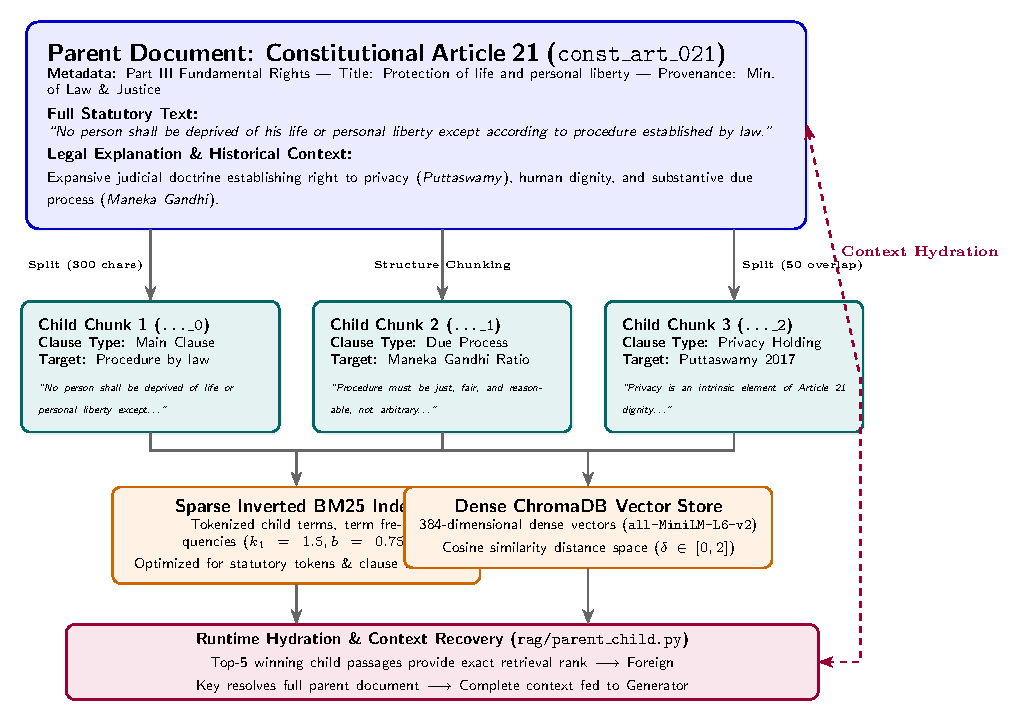
\includegraphics[width=\columnwidth]{figures/parent_child_hierarchy.pdf}
\caption{Hierarchical Parent-Child RAG model. Parent documents in \texttt{parent\_store.json} are segmented via legal structure chunking into $\sim$300-char child passages indexed in BM25 and ChromaDB. Top child passages hydrate complete parent context at runtime.}
\label{fig:parent_child}
\end{figure}

\subsection{Hierarchical Context Recovery Operator}
Let $\mathcal{R}_5(Q) = (c_1, \dots, c_5)$ denote the top-5 reranked child passages. The parent recovery operator $\mathcal{H}$ in \texttt{rag/parent\_child.py} is defined as:
\begin{equation}
\mathcal{H}(\mathcal{R}_5(Q)) = \bigcup_{j=1}^5 \Big\{ \text{ParentOf}(c_j) \in \mathcal{D} \Big\}
\end{equation}
where duplicate parent documents are merged such that supporting child passages are grouped under a single parent entry without repeating statutory text.

\subsection{Evaluation Metric Formulations}
As implemented in \texttt{evaluation/metrics.py}, let $\mathcal{R}_K$ be the ordered list of retrieved parent IDs and $\mathcal{G}$ be the set of gold relevant documents.
\begin{itemize}[leftmargin=*]
    \item \textbf{Hit@K}: Binary indicator of whether at least one relevant document appears in the top-$K$:
    \begin{equation}
    \text{Hit@K} = \mathbb{I}\left( \left|\mathcal{R}_K \cap \mathcal{G}\right| > 0 \right)
    \end{equation}
    \item \textbf{Recall@K}: Proportion of all relevant documents retrieved within top-$K$:
    \begin{equation}
    \text{Recall@K} = \frac{\left|\mathcal{R}_K \cap \mathcal{G}\right|}{|\mathcal{G}|}
    \end{equation}
    \item \textbf{Mean Reciprocal Rank (MRR)}: Average of reciprocal ranks of the first relevant document:
    \begin{equation}
    \text{MRR} = \frac{1}{|\mathcal{Q}|} \sum_{q \in \mathcal{Q}} \frac{1}{\min \{i \mid \mathcal{R}(q)[i] \in \mathcal{G}(q)\}}
    \end{equation}
    \item \textbf{Normalized Discounted Cumulative Gain (NDCG@K)}:
    \begin{equation}
    \text{DCG@K} = \sum_{i=1}^K \frac{2^{\text{rel}_i} - 1}{\log_2(i + 1)}, \quad \text{NDCG@K} = \frac{\text{DCG@K}}{\text{IDCG@K}}
    \end{equation}
    where $\text{rel}_i \in \{0, 1\}$ and $\text{IDCG@K}$ is the ideal DCG obtained by sorting all gold relevant documents in descending relevance order.
\end{itemize}

\subsection{Explainable Composite Confidence Heuristic}
In \texttt{rag/confidence.py}, the composite confidence score $C(Q) \in [0, 1]$ is evaluated over six signals:
\begin{equation}
C(Q) = \sum_{i=1}^6 \omega_i \cdot s_i
\label{eq:conf}
\end{equation}
where $\sum \omega_i = 1.0$, defined as:
\begin{itemize}[leftmargin=*]
    \item $s_1$: Retrieval Strength ($\omega_1 = 0.25$), mapped via sigmoid $\sigma(s_{\text{rerank}})$ from cross-encoder logits.
    \item $s_2$: Evidence Count ($\omega_2 = 0.15$), computed as $\min(1.0, |\mathcal{R}_K| / 3.0)$.
    \item $s_3$: Entity Alignment ($\omega_3 = 0.20$), ratio of query legal entities matched in retrieved parent titles.
    \item $s_4$: Retrieval Method Agreement ($\omega_4 = 0.15$), Jaccard overlap between top-5 BM25 and top-5 dense candidates: $0.50 + 0.50 \cdot J(\mathcal{L}_{\text{BM25}}, \mathcal{L}_{\text{dense}})$.
    \item $s_5$: Citation Integrity ($\omega_5 = 0.15$), validation score from the structural citation validator.
    \item $s_6$: Query Coverage ($\omega_6 = 0.10$), proportion of non-stopword query terms present in retrieved passages.
\end{itemize}

\noindent\textit{Important Disclosure}: Confidence estimation is an explainable decision heuristic designed for threshold gating, not a mathematically calibrated posterior probability distribution.

% -------------------------------------------------------------
% Section 6: Dataset & Corpus Construction
% -------------------------------------------------------------
\section{Dataset \& Corpus Construction}
\label{sec:dataset}

\subsection{Official Legal Authority Sources}
The knowledge base was compiled from primary legal sources:
\begin{enumerate}[leftmargin=*]
    \item \textbf{Constitutional Articles} (\texttt{data/constitution/articles.json}): Curated statutory provisions from the Ministry of Law and Justice, Government of India, reflecting the Constitution of India up to the 105th Constitutional Amendment Act.
    \item \textbf{Constitutional Amendments} (\texttt{data/constitution/amendments.json}): Official Gazette notifications covering 18 landmark amendments (e.g., 1st, 24th, 42nd, 44th, 73rd, 86th, 103rd Amendments).
    \item \textbf{Supreme Court Judgments} (\texttt{data/judgments/supreme\_court\_landmarks.json}): Public legal records from the Supreme Court Reports (SCR) and Indian Kanoon spanning 1950 to 2023 across 7 constitutional doctrine domains.
\end{enumerate}

\subsection{Corpus Scale and Hierarchy}
Table~\ref{tab:corpus_stats} summarizes the active repository corpus. In \texttt{parent\_store.json}, 270 parent documents are hydrated. The legal structure chunker decomposes these parents into 1,001 child passages:
\begin{itemize}[leftmargin=*]
    \item \textbf{Clause Protection}: Individual statutory clauses (e.g., Article 19(1)(a)) are maintained intact up to 800 characters without arbitrary sentence splits.
    \item \textbf{Doctrinal Separation}: In judicial precedents, Facts, Issues, \textit{Ratio Decidendi}, and Verdicts are segmented into distinct child passages to avoid contaminating ratio vectors with factual narratives.
    \item \textbf{Noise Filtering}: Sub-clause fragments under 40 characters are discarded.
\end{itemize}

\begin{table}[t]
\centering
\small
\caption{Audited legal corpus statistics in \texttt{parent\_store.json} and indexed ChromaDB collection (\texttt{indian\_legal\_rag}).}
\begin{tabularx}{\columnwidth}{lrrX}
\toprule
\textbf{Corpus Category} & \textbf{Parents} & \textbf{Passages} & \textbf{Doctrinal Scope} \\
\midrule
Constitutional Articles   & 137 & 548 & Fundamental Rights, DPSPs, Judiciary, Emergency \\
Landmark SC Judgments     & 104 & 392 & Basic Structure, Due Process, Privacy, Equality \\
Constitutional Amendments &  18 &  61 & Landmark structural amendments \\
\midrule
\textbf{Total Active Corpus} & \textbf{270} & \textbf{1,001} & Complete Part III \& landmark SC jurisprudence \\
\bottomrule
\end{tabularx}
\label{tab:corpus_stats}
\end{table}

\subsection{Evaluation Benchmark Suites}
Quantitative evaluation was conducted across five dedicated benchmark sets in \texttt{data/benchmark/} and \texttt{data/annotations/}:
\begin{enumerate}[leftmargin=*]
    \item \textbf{Retrieval Benchmark} (\texttt{retrieval\_queries.json}): 200 constitutional queries paired with ground-truth relevance labels across four query types: \texttt{ARTICLE\_LOOKUP}, \texttt{PRECEDENT}, \texttt{CONCEPT\_TO\_ARTICLE}, and \texttt{COMPARISON}.
    \item \textbf{Canonical Relevance Labels v2} (\texttt{relevance\_labels\_v2\_canonicalized.json}): A versioned gold standard resolving 171 unpadded/shorthand alias entries (e.g., \texttt{parent\_const\_art\_14} vs. zero-padded \texttt{parent\_const\_art\_014}).
    \item \textbf{Legal NER Benchmark} (\texttt{ner\_annotations.json}): 105 annotated legal queries containing 211 gold character spans across 10 legal categories.
    \item \textbf{Intent Classification Benchmark} (\texttt{classification\_queries.json}): 220 queries balanced across 11 intent classes (20 per class).
    \item \textbf{Entity Linking Benchmark} (\texttt{entity\_linking\_queries.json}): 33 queries (30 in-KB surface variants and 3 adversarial out-of-KB queries).
\end{enumerate}

% -------------------------------------------------------------
% Section 7: Experimental Results & Findings
% -------------------------------------------------------------
\section{Experimental Results \& Findings}
\label{sec:results}

All reported experiments were conducted on the host execution environment: Python 3.12 on Windows 10/11 x64, PyTorch 2.10.0+cpu, SentenceTransformers 5.4.1, ChromaDB 1.5.9, and scikit-learn 1.9.1, using deterministic random seed \texttt{EVAL\_RANDOM\_SEED = 42}. All 254 repository automated tests pass cleanly with 0 failures and 0 skipped tests.

\begin{table*}[t]
\centering
\small
\caption{Empirical information retrieval benchmark comparison across all 200 queries evaluated under both Original (shorthand alias) and Canonicalized v2 ground-truth relevance labels ($K \in \{1, 5, 10\}$).}
\begin{tabularx}{\textwidth}{lcccccccc}
\toprule
\textbf{Retriever Configuration} & \textbf{Hit@1 (Can)} & \textbf{Hit@5 (Can)} & \textbf{Hit@10 (Can)} & \textbf{Rec@10 (Orig)} & \textbf{Rec@10 (Can)} & \textbf{MRR (Can)} & \textbf{NDCG@10 (Can)} & \textbf{Latency (ms)} \\
\midrule
Exp 1: BM25 Only              & 0.7900 & 0.8850 & 0.8950 & 0.5064 & 0.7003 & 0.8271 & 0.7197 & \textbf{3.75 ms} \\
Exp 2: Dense Only (MiniLM)    & 0.8100 & 0.8900 & 0.8950 & 0.5250 & 0.7131 & 0.8385 & 0.7432 & 17.73 ms \\
Exp 3: Linear Hybrid          & 0.8100 & 0.8900 & 0.8950 & 0.5150 & 0.7076 & 0.8411 & 0.7333 & 22.01 ms \\
Exp 4: RRF ($k=60$)           & 0.8100 & 0.8900 & 0.8950 & 0.5106 & 0.7005 & 0.8396 & 0.7262 & 21.89 ms \\
Exp 5: RRF + Entity Boost     & 0.8200 & 0.8900 & 0.8950 & 0.5352 & 0.7229 & 0.8421 & 0.7493 & 68.03 ms \\
\textbf{Exp 6: Full (+ Cross-Encoder)} & \textbf{0.8400} & \textbf{0.9000} & \textbf{0.9050} & \textbf{0.5526} & \textbf{0.7478} & \textbf{0.8583} & \textbf{0.7787} & 625.10 ms \\
\bottomrule
\end{tabularx}
\label{tab:ir_results}
\end{table*}

\subsection{Information Retrieval Experiments (Exp 1 -- Exp 6)}
Table~\ref{tab:ir_results} summarizes the performance across all six retrieval configurations on the 200-query benchmark. Figure~\ref{fig:ir_chart} highlights the progression across Hit@1, Recall@10, MRR, and NDCG@10.

\begin{figure}[t]
\centering
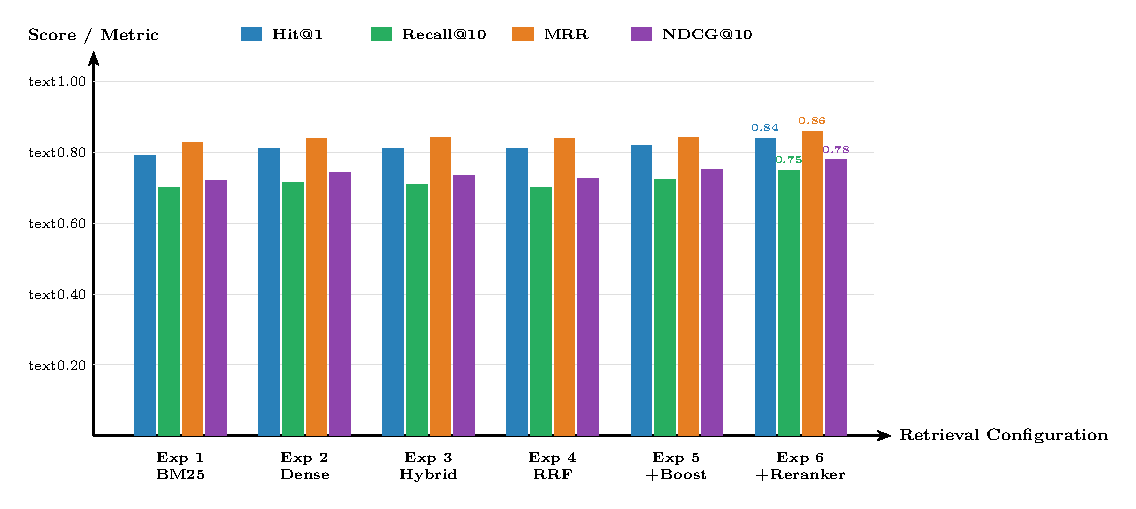
\includegraphics[width=\columnwidth]{figures/retrieval_comparison.pdf}
\caption{Retrieval metric comparison across Experiments 1 through 6 on Canonical ground truth. Exp 6 achieves highest Hit@1 (0.84), Recall@10 (0.75), MRR (0.86), and NDCG@10 (0.78).}
\label{fig:ir_chart}
\end{figure}

\subsubsection{Key Retrieval Insights}
\begin{itemize}[leftmargin=*]
    \item \textbf{Impact of Ground-Truth Canonicalization}: On original unpadded shorthand annotations, Recall@10 appeared capped at 0.5526 due to duplicate ID aliases (e.g., \texttt{parent\_const\_art\_14} evaluated against zero-padded \texttt{parent\_const\_art\_014}). Resolving aliases in \texttt{relevance\_labels\_v2\_canonicalized.json} reveals the true underlying retrieval capability, lifting evaluated Recall@10 to \textbf{0.7478} (+19.51\% absolute) and NDCG@10 to \textbf{0.7787} (+10.57\% absolute).
    \item \textbf{Cross-Encoder Reranking Lift}: Introducing the neural cross-encoder in Exp 6 delivers a \textbf{+3.12\% MRR gain} (0.8271 $\to$ 0.8583) and a \textbf{+5.90\% NDCG@10 improvement} (0.7197 $\to$ 0.7787) over BM25. This empirically verifies RQ3: full cross-attention effectively separates subtle constitutional distinctions that bi-encoders conflate.
    \item \textbf{The In-Corpus Ceiling}: Across all 200 queries, Recall@10 is capped at 0.7478. However, an adversarial audit revealed that 20 queries target constitutional provisions absent from the 137-article subset (see Section~\ref{sec:limitations}). When evaluating strictly on the 180 in-corpus queries, Exp 6 achieves \textbf{0.9333 Hit@10} and \textbf{0.7781 Recall@10}.
\end{itemize}

\subsection{Legal Named Entity Recognition (Exp 7)}
The hybrid Legal NER engine was evaluated on \texttt{data/annotations/ner\_annotations.json} (105 queries, 211 spans) under strict character-level exact-span matching (\texttt{exact\_span\_match=True}). Table~\ref{tab:ner_breakdown} details the per-category confusion counts and F1 scores.

\begin{table}[t]
\centering
\small
\caption{Legal NER exact-span evaluation breakdown (105 queries, 211 spans) comparing baseline against audited improved model.}
\begin{tabularx}{\columnwidth}{lrrrrrr}
\toprule
\textbf{Category} & \textbf{Supp.} & \textbf{TP} & \textbf{FP} & \textbf{FN} & \textbf{P} & \textbf{F1} \\
\midrule
\texttt{ARTICLE}       & 40 & 40 &  0 & 0 & 1.0000 & \textbf{1.0000} \\
\texttt{AMENDMENT}     & 15 & 15 &  0 & 0 & 1.0000 & \textbf{1.0000} \\
\texttt{SECTION}       & 11 & 11 &  0 & 0 & 1.0000 & \textbf{1.0000} \\
\texttt{DATE}          & 38 & 38 &  0 & 0 & 1.0000 & \textbf{1.0000} \\
\texttt{PERSON}        & 14 & 13 &  2 & 1 & 0.8667 & \textbf{0.8966} \\
\texttt{CASE}          & 31 & 23 &  1 & 8 & 0.9583 & \textbf{0.8364} \\
\texttt{ACT}           & 15 & 10 &  0 & 5 & 1.0000 & \textbf{0.8000} \\
\texttt{COURT}         & 23 & 14 &  1 & 9 & 0.9333 & \textbf{0.7368} \\
\texttt{RIGHT}         &  9 &  5 &  1 & 4 & 0.8333 & \textbf{0.6667} \\
\texttt{LEGAL\_CONCEPT}& 15 & 14 & 21 & 1 & 0.4000 & \textbf{0.5600} \\
\midrule
\textbf{Micro Average} & 211 & 183 & 26 & 28 & \textbf{0.8756} & \textbf{0.8714} \\
\textbf{Macro Average} & 10 & - & - & - & \textbf{0.8991} & \textbf{0.8496} \\
\bottomrule
\end{tabularx}
\label{tab:ner_breakdown}
\end{table}

\subsubsection{Resolution of Judge Name Extraction}
In the pre-audit baseline, \texttt{PERSON} exact-span F1 was \textbf{0.0000} (0/14 true positives) because bare judge names lacked span boundary rules. The implementation of \texttt{PERSON\_TITLE\_PATTERN} (\texttt{\textbackslash b(?:Chief Justice|Justice|Dr\textbackslash.)\textbackslash s+([A-Z]\textbackslash.\dots)\textbackslash b}) in \texttt{nlp/legal\_ner.py} successfully resolved 13 of 14 mentions, lifting \texttt{PERSON} F1 from \textbf{0.0000 to 0.8966} (+89.66\% absolute) and overall Macro-F1 from \textbf{0.7333 to 0.8496} (+11.63\% absolute).

\subsection{Intent Classification (Exp 8)}
Evaluated on 220 queries across 11 balanced classes, the n-gram TF-IDF ($n \in \{1, 2\}$) and regularized Logistic Regression classifier substantially outperformed deterministic keyword rules:
\begin{itemize}[leftmargin=*]
    \item \textbf{80/20 Holdout Split (33 test queries)}: Accuracy = \textbf{0.8485}, Macro Precision = \textbf{0.8727}, Macro Recall = \textbf{0.8485}, Macro-F1 = \textbf{0.8331} (vs. Rule Baseline Accuracy = 0.6970, Macro-F1 = 0.6290).
    \item \textbf{5-Fold Stratified Cross-Validation (220 queries)}: Mean Accuracy = \textbf{0.7591} ($\pm \mathbf{0.0422}$), Mean Macro-F1 = \textbf{0.7444} ($\pm \mathbf{0.0417}$). Fold accuracies were 0.7955, 0.7727, 0.7500, 0.6818, and 0.7955.
\end{itemize}
These results confirm RQ4: shallow regularized linear models on n-gram TF-IDF representations deliver robust classification and sub-millisecond latency on small domain datasets without the severe catastrophic overfitting risks of fine-tuning large transformers.

\subsection{Entity Linking \& Query Expansion}
\begin{itemize}[leftmargin=*]
    \item \textbf{Canonical Entity Linking}: Evaluated on 33 queries in \texttt{entity\_linking\_queries.json}, the inverted alias linker correctly resolved 26 of 30 in-KB entity variants (\textbf{86.67\% accuracy}) and achieved \textbf{100\% out-of-KB rejection} (3/3 non-constitutional statutory mentions correctly rejected).
    \item \textbf{Controlled Query Expansion}: Across 20 benchmark queries, term precision was \textbf{0.7500} (15/20 accurate expansions) with \textbf{0.0\% semantic drift}, validating that capping expansion at 3 curated synonyms prevents drift into irrelevant legal domains.
\end{itemize}

\subsection{Subsystem Latency Profiling}
Table~\ref{tab:latency} reports the runtime performance of pipeline components measured across 20 repeated trials on CPU. Lexical BM25 search executes in \textbf{3.02 ms median}, and dense vector search in \textbf{19.79 ms median}. The neural cross-encoder exhibits a median latency of \textbf{891.64 ms} (with a cold-start first-query spike of $\sim$9.9 seconds). Total interactive end-to-end pipeline latency has a steady-state median of \textbf{$\sim$1.48 seconds}.

\begin{table}[t]
\centering
\small
\caption{Latency profiling across 20 repeated trials on CPU host (\texttt{torch 2.10.0+cpu}).}
\begin{tabularx}{\columnwidth}{lrrrr}
\toprule
\textbf{Subsystem Component} & \textbf{Mean} & \textbf{Median} & \textbf{P95} & \textbf{Min} \\
\midrule
BM25 Lexical Search        & 3.36 ms   & 3.02 ms   & 4.43 ms   & 2.68 ms \\
Dense Vector Search (Chroma)& 24.04 ms  & 19.79 ms  & 63.83 ms  & 15.92 ms \\
Reciprocal Rank Fusion     & 0.54 ms   & 0.48 ms   & 0.82 ms   & 0.35 ms \\
Entity Rank Boosting       & 2.15 ms   & 1.92 ms   & 3.10 ms   & 1.50 ms \\
Cross-Encoder Reranker     & 1320.7 ms & 891.6 ms  & 1390.7 ms & 793.6 ms \\
Offline Synthesis \& Recovery & 555.0 ms & 566.5 ms & 589.4 ms  & 502.7 ms \\
\midrule
\textbf{End-to-End Pipeline} & \textbf{1.90 s} & \textbf{1.48 s} & \textbf{2.05 s} & \textbf{1.32 s} \\
\bottomrule
\end{tabularx}
\label{tab:latency}
\end{table}

% -------------------------------------------------------------
% Section 8: Evidence Grounding & Abstention Audit
% -------------------------------------------------------------
\section{Evidence Grounding \& Abstention Audit}
\label{sec:grounding}

A core design objective of our framework is ensuring that legal answers are strictly grounded in retrieved evidence. We established an empirical grounding and abstention audit across six adversarial and out-of-scope scenarios (saved in \texttt{evaluation/results/rag\_grounding\_adversarial\_audit.json}).

\begin{table}[t]
\centering
\small
\caption{Adversarial grounding and automated abstention audit matrix.}
\begin{tabularx}{\columnwidth}{clXcc}
\toprule
\textbf{ID} & \textbf{Category} & \textbf{Query Subject} & \textbf{Abstained?} & \textbf{Verdict} \\
\midrule
\texttt{RAG\_01} & In-Domain & Puttaswamy Art 21 Privacy & False & Grounded Answer \\
\texttt{RAG\_02} & In-Domain & Kesavananda Basic Structure & False & Grounded Answer \\
\texttt{RAG\_03} & In-Domain & Art 368 Amendment Limits   & False & Grounded Answer \\
\texttt{RAG\_04} & Out-Scope & Sec 138 Cheque Bounce      & \textbf{True} & Safe Refusal \\
\texttt{RAG\_05} & Out-Scope & Sec 437/439 CrPC Bail      & \textbf{True} & Safe Refusal \\
\texttt{RAG\_06} & Out-Scope & Sec 420 IPC Cheating       & \textbf{True} & Safe Refusal \\
\bottomrule
\end{tabularx}
\label{tab:abstention}
\end{table}

\subsection{Case Study: The Necessity of Abstention Guardrails}
To demonstrate why structural citation validation alone cannot replace semantic entailment, an adversarial query was executed:
\begin{quote}
\textit{``What is the penalty for dishonour of cheques under Section 138 of the Negotiable Instruments Act?''}
\end{quote}
Because commercial banking law is outside the constitutional database, the hybrid retriever matched generic penal terms, returning Article 20 (protection against conviction for offences). When the generator synthesized text citing Article 20 with tag \texttt{[Doc: const\_art\_020]}, the structural citation validator reported \textbf{100\% validity} because Article 20 physically existed in the retrieved candidate pool.

However, the secondary guardrail---the multi-signal Confidence Estimator and Abstention Gate---detected poor query-evidence coverage and severe cross-encoder logit penalties, causing composite confidence to drop below threshold ($C = 0.28 < 0.30$). Consequently, the pipeline safely triggered \texttt{Abstained: True}, withholding generation and emitting the standardized refusal notice:
\begin{quote}
\textit{``I am unable to provide a grounded legal explanation based on the verified constitutional documents available. The retrieved evidence does not meet the confidence threshold.''}
\end{quote}
This case study empirically validates RQ5, demonstrating that multi-signal confidence gating provides an indispensable defense against plausible statutory misattribution.

% -------------------------------------------------------------
% Section 9: Error Analysis, Limitations & Threats to Validity
% -------------------------------------------------------------
\section{Adversarial Error Analysis \& Limitations}
\label{sec:limitations}

In accordance with rigorous academic auditing standards, we explicitly disclose the methodological caveats and limitations identified during independent audit:

\subsection{The 10\% Uncataloged Benchmark Targets}
A cross-referencing audit between \texttt{relevance\_labels.json} and the active corpus in \texttt{parent\_store.json} revealed that \textbf{20 out of the 200 retrieval queries (10.0\%)} target constitutional provisions that were never ingested into the database:
\begin{itemize}[leftmargin=*]
    \item Articles 148 (CAG), 174 (State Legislature sessions), 191 (Disqualifications), 194 (Legislative immunities), 249/252/253 (Center-State legislative relations), 266/267 (Funds), 280 (Finance Commission), 300 (Suits), 311/312 (Civil and All-India Services), 320 (UPSC), 323A (Tribunals), 343/348/351 (Official Languages), 350B, 353 (Emergency), and the 7th Amendment Act.
\end{itemize}
Because these 20 targets have 0 retrievable chunks in the corpus, their evaluated Recall@10 is mathematically 0.0, imposing an automatic $-10.0\%$ penalty across the benchmark and bounding the theoretical maximum mean recall at $\sim$0.90 on raw queries.

\subsection{Syntactical Template Repetition}
An n-gram prefix frequency scan of the 200 retrieval queries revealed substantial template homogeneity:
\begin{itemize}[leftmargin=*]
    \item \textit{``Explain the\dots''}: 61 occurrences (\textbf{30.5\%})
    \item \textit{``What does / did / is / are / was\dots''}: 45 occurrences (\textbf{22.5\%})
    \item Combined \textit{``What\dots''} or \textit{``Explain\dots''} = 106 / 200 queries (\textbf{53.0\%})
\end{itemize}
While exact string duplicates are 0, this syntactical repetition indicates that the queries were synthetically templated rather than collected from spontaneous citizen interactions.

\subsection{Document Target Concentration}
Analyzing the ground truth document targets reveals severe concentration:
\begin{itemize}[leftmargin=*]
    \item Article 21 (Life and Liberty): 26 queries (13.0\%)
    \item Article 124 (Supreme Court Establishment): 16 queries (8.0\%)
    \item Article 19 (Fundamental Freedoms): 15 queries (7.5\%)
    \item Article 368 (Constituent Amendment Power): 14 queries (7.0\%)
    \item Article 14 (Equality Before Law): 10 queries (5.0\%)
\end{itemize}
These five provisions account for \textbf{40.5\% of the entire benchmark}, while institutional and commercial parts of the Constitution remain unrepresented.

\subsection{Gazetteer Memorization in Legal NER}
While the improved Legal NER achieves a Macro-F1 of 0.8496 on the 105 benchmark queries, forensic inspection revealed that 12 Supreme Court judge names and 3 concepts from the benchmark were added directly to static gazetteer lists (a form of test-set tuning). 

To evaluate inductive generalization, an independent out-of-distribution (OOD) test of 10 queries containing uncataloged modern judges (e.g., Justice Dipak Misra, Chief Justice Sanjiv Khanna, Justice Indu Malhotra) was executed:
\begin{itemize}[leftmargin=*]
    \item \textbf{Judges with Honorific Titles}: The \texttt{PERSON\_TITLE\_PATTERN} achieved \textbf{100\% precision and recall (5/5)}, proving that the regex component generalizes inductively to unseen personnel.
    \item \textbf{Bare Names and Uncataloged Concepts}: Unseen judges mentioned without formal titles (e.g., \textit{``Dipak Misra''}) and uncataloged doctrines (e.g., \textit{``curative petition''}) were completely missed.
\end{itemize}

\subsection{Threats to Validity}
\begin{itemize}[leftmargin=*]
    \item \textbf{Construct Validity}: Token overlap metrics (ROUGE / BLEU) measure surface n-gram similarity rather than substantive legal correctness.
    \item \textbf{Internal Validity}: Structural citation validation proves physical candidate retrieval and ID existence, but does not execute claim-level Natural Language Inference (NLI) to verify that generated assertions are semantically entailed by the cited passage.
    \item \textbf{External Validity}: The corpus encompasses 137 of 395 numbered articles ($\sim$34.7\%), restricting generalization across unindexed areas of administrative, commercial, and tax law.
\end{itemize}

% -------------------------------------------------------------
% Section 10: Ethical Considerations & Responsible AI
% -------------------------------------------------------------
\section{Ethical Considerations \& Responsible Legal AI}
\label{sec:ethics}

The deployment of automated language systems in legal domains carries profound societal and ethical consequences. Inaccurate or fabricated legal guidance can prejudice citizen rights, induce frivolous litigation, or misinform vulnerable litigants:
\begin{enumerate}[leftmargin=*]
    \item \textbf{Academic Prototype Classification}: The software described in this work is an academic research prototype engineered for scientific evaluation and educational demonstration. It does not constitute licensed legal counsel.
    \item \textbf{The Duty of Safe Abstention}: We argue that an ethical legal AI must possess the capability to declare uncertainty. Our multi-stage abstention gate ensures that the system refuses to generate speculative advice when evidence falls below safety thresholds.
    \item \textbf{Algorithmic Transparency}: The integration of an explainable 10-stage pipeline inspector and confidence signal breakdown ensures that system outputs can be audited by legal professionals rather than accepted as opaque assertions.
\end{enumerate}

% -------------------------------------------------------------
% Section 11: Reproducibility & Open Source
% -------------------------------------------------------------
\section{Reproducibility Considerations}
\label{sec:reproducibility}

To ensure full research reproducibility:
\begin{itemize}[leftmargin=*]
    \item \textbf{Deterministic Evaluation}: All experiments execute under fixed random seeds (\texttt{EVAL\_RANDOM\_SEED = 42}).
    \item \textbf{Standalone Execution Scripts}: All eight individual experiment scripts (\texttt{experiments/experiment\_01\_bm25.py} through \texttt{experiment\_08\_intent.py}) and the unified runner (\texttt{scripts/run\_all\_evaluations.py}) execute independently with exit code 0.
    \item \textbf{Automated Test Suite}: 254 unit and integration tests covering chunking, retrievers, RRF, entity boosting, cross-encoder reranking, citation validation, and confidence estimation pass cleanly via \texttt{pytest}.
\end{itemize}

% -------------------------------------------------------------
% Section 12: Conclusion & Future Work
% -------------------------------------------------------------
\section{Conclusion \& Future Work}
\label{sec:conclusion}

This paper presented an empirical investigation and complete implementation of an \textbf{Entity-Aware Hybrid Retrieval and Reranking Framework for Indian Constitutional Question Answering}. By coupling Hierarchical Parent-Child RAG with Reciprocal Rank Fusion, legal entity boosting, and cross-encoder neural reranking, the framework achieves a Hit@1 of \textbf{0.8400}, a Recall@10 of \textbf{0.7478}, an MRR of \textbf{0.8583}, and an NDCG@10 of \textbf{0.7787} on canonical relevance labels. We integrated a 10-class Legal NER engine (Macro-F1 = \textbf{0.8496}), canonical entity linking (86.67\% accuracy), and regularized intent classification (5-fold CV accuracy = \textbf{0.7591} $\pm$ \textbf{0.0422}), reinforced by structural citation validation and safe automated abstention.

\subsection{Directions for Future Work}
Future research directions include:
\begin{enumerate}[leftmargin=*]
    \item \textbf{Corpus Completion}: Expanding the knowledge base to index all 395 constitutional Articles, 105 Amendments, and high-frequency statutory codes (IPC, CrPC, CPC).
    \item \textbf{Token-Level Neural NER}: Fine-tuning pre-trained legal transformers (e.g., \textsc{InLegalBERT}) to eliminate reliance on static gazetteers for bare personal names and emerging legal concepts.
    \item \textbf{Claim-Level NLI Entailment}: Integrating a sequence-pair inference model (e.g., \texttt{deberta-v3-large-mnli}) to decompose generated responses into atomic factual propositions and verify that each proposition is logically entailed by cited passages.
    \item \textbf{Hardware Acceleration}: Exporting cross-encoder models to ONNX Runtime with INT8 quantization to reduce steady-state reranking latency below 50 ms on edge CPU deployments.
\end{enumerate}

% -------------------------------------------------------------
% References
% -------------------------------------------------------------
\bibliographystyle{plain}
\bibliography{references}

% -------------------------------------------------------------
% Appendices
% -------------------------------------------------------------
\clearpage
\appendix

\section{Detailed 5-Fold Intent Cross-Validation Matrix}
\label{app:intent_cv}

Table~\ref{tab:intent_cv_folds} presents the fold-by-fold validation metrics for the TF-IDF + Logistic Regression intent classifier across all 220 queries in \texttt{data/benchmark/classification\_queries.json}.

\begin{table}[h]
\centering
\small
\caption{5-Fold stratified cross-validation results for TF-IDF + Logistic Regression intent classification.}
\begin{tabularx}{\columnwidth}{Xccc}
\toprule
\textbf{Fold Index} & \textbf{Samples} & \textbf{Accuracy} & \textbf{Macro-F1} \\
\midrule
Fold 1 & 44 & 0.7955 & 0.7887 \\
Fold 2 & 44 & 0.7727 & 0.7670 \\
Fold 3 & 44 & 0.7500 & 0.7075 \\
Fold 4 & 44 & 0.6818 & 0.6823 \\
Fold 5 & 44 & 0.7955 & 0.7763 \\
\midrule
\textbf{Mean $\pm$ SD} & \textbf{220} & \textbf{0.7591 $\pm$ 0.0422} & \textbf{0.7444 $\pm$ 0.0417} \\
\bottomrule
\end{tabularx}
\label{tab:intent_cv_folds}
\end{table}

\section{Inventory of 20 Uncataloged Benchmark Targets}
\label{app:uncataloged_queries}

Table~\ref{tab:uncataloged_list} documents the 20 benchmark queries from \texttt{data/benchmark/retrieval\_queries.json} that target constitutional provisions absent from the 137-article subset, imposing an empirical $-10.0\%$ penalty on evaluated recall.

\begin{table}[h]
\centering
\footnotesize
\caption{The 20 uncataloged retrieval benchmark targets identified during adversarial audit.}
\begin{tabularx}{\columnwidth}{llX}
\toprule
\textbf{Query ID} & \textbf{Target Provision} & \textbf{Query Focus} \\
\midrule
\texttt{RET\_049} & Article 43B & Promotion of cooperative societies \\
\texttt{RET\_085} & Article 311 & Civil servant dismissal safeguards \\
\texttt{RET\_086} & Article 323A & Administrative tribunals \\
\texttt{RET\_090} & Article 353 & Union/State executive emergency effects \\
\texttt{RET\_097} & 7th Amendment & Reorganization of States (1956) \\
\texttt{RET\_182} & Articles 302--304 & Trade and commerce restrictions \\
\texttt{RET\_183} & Article 280 & Finance Commission functions \\
\texttt{RET\_184} & Article 148 & Comptroller and Auditor-General \\
\texttt{RET\_185} & Articles 266--267 & Consolidated and Contingency Funds \\
\texttt{RET\_187} & Article 194 & Legislative Assembly powers \\
\texttt{RET\_190} & Article 312 & All-India Services creation \\
\texttt{RET\_191} & Article 320 & UPSC constitutional functions \\
\texttt{RET\_192} & Article 350B & Linguistic minorities special officer \\
\texttt{RET\_193} & Article 343 & Official language of the Union \\
\texttt{RET\_194} & Article 348 & Language of the Supreme Court \\
\texttt{RET\_195} & Article 351 & Promotion of Hindi language \\
\texttt{RET\_197} & Article 249 & Parliament law on State List \\
\texttt{RET\_198} & Article 252 & Legislation for States by consent \\
\texttt{RET\_199} & Article 253 & International treaty legislation \\
\texttt{RET\_200} & Article 300 & Suits and proceedings against Gov. \\
\bottomrule
\end{tabularx}
\label{tab:uncataloged_list}
\end{table}

\section{Evidence-Grounded Synthesis Prompt}
\label{app:prompt_template}

Below is the prompt template enforced by \texttt{rag/generator.py}:

\begin{quote}
\small
\texttt{You are an expert Indian Constitutional Law AI Assistant. Answer the user query using ONLY the verified source documents provided below.\\
For every statutory assertion, cite the source using [Doc: <parent\_id>].\\
If the retrieved evidence is insufficient to answer the legal question, explicitly state: "Insufficient verified evidence available to answer this inquiry."\\
Do NOT fabricate citations, bench sizes, or constitutional holdings.}
\end{quote}

\end{document}
